\documentclass{article}
\usepackage{graphicx}
\usepackage{subcaption}
\usepackage[margin=1in]{geometry}

\begin{document}

\begin{figure}
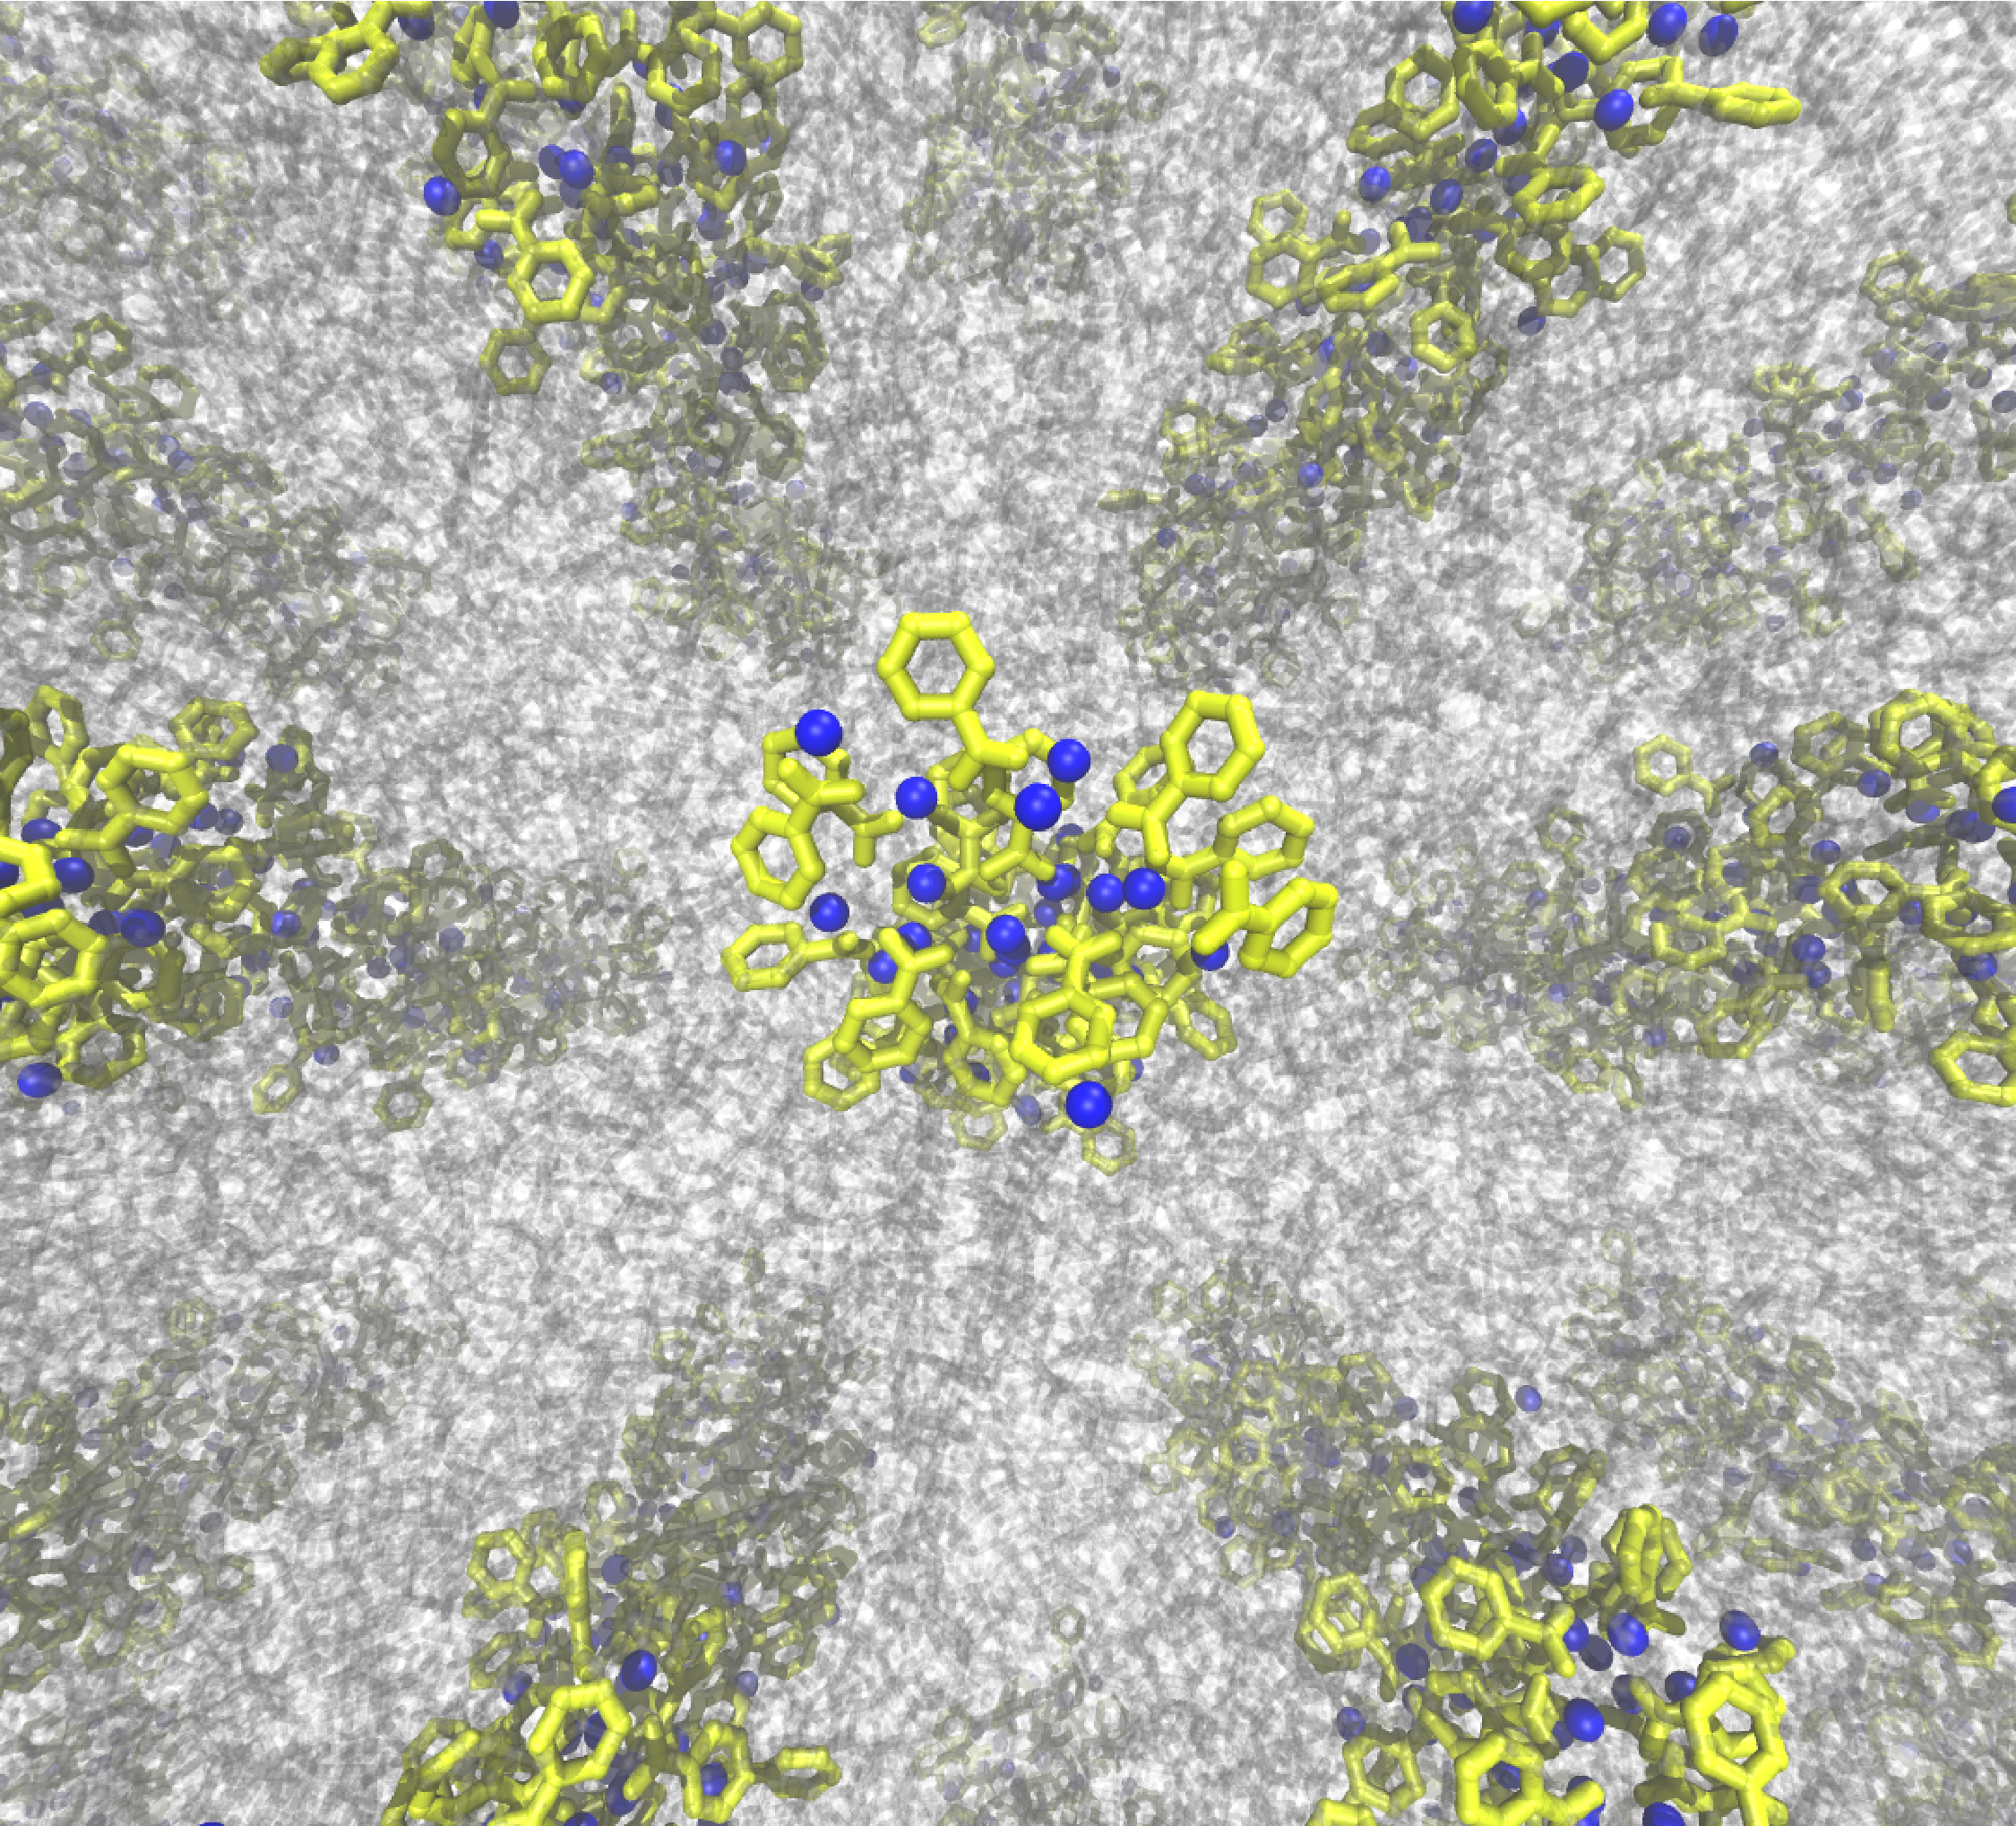
\includegraphics[width=\textwidth]{toc_image_final.pdf}
\caption*{We studied the atomistic structure of a lyotropic liquid crystal
	(LLC) membrane using molecular dynamics simulations run for hundreds of
	nanoseconds enabled by Bridges GPU nodes. We learned that the membrane pores
	(represented by blue sodium ions and yellow LLC monomer head groups above) are
	dense with a gradual transition from hydrophilic to hydrophobic character as
	distance from the pore center increases. We will use our model, which has been
	validated with experimental studies, in order to characterize transport of
	small molecules inside the nanopores so we can learn how to design new LLC
	membranes for solute-specific separations.} 
\end{figure}
		
\end{document}
